\section{Design and Implementation}

\subsection{Platforms and Language Choice}

Since this application is built for Android tablets, we had to either write our application natively in Java with the Android SDK, or use a middleware platform. We ultimately chose the native approach due to several considerations. We needed to access external sdk’s and libraries that may not have been supported by any given middleware platform. We also did not require the major benefit of using such a platform (cross-platform compatibility, eg. with iOS) and also many of the better
ones are neither open source nor free. 
Once we had decided to go with native java, we had to choose a computer vision library. The obvious choice was to go with OpenCV as it is widely used, open source, powerful and has a variety of useful features. We also ended up using a library called FileDialog (CIT) for our file dialogs, and Android MIDI library to generate our MIDIs.

\subsection{Application Layout}

Once the language and libraries were chosen, we decided to start the design of the application. This original design has only suffered from minor changes until the end. There are 3 main parts: 
\begin{enumerate}
\item{The Android application}
\item{Music detection}
\item{Interpreting and playing back the music}
\end{enumerate}

(IMAGE)


\subsection{The Android Application}

            \begin{figure}[ht!]
                \centering
                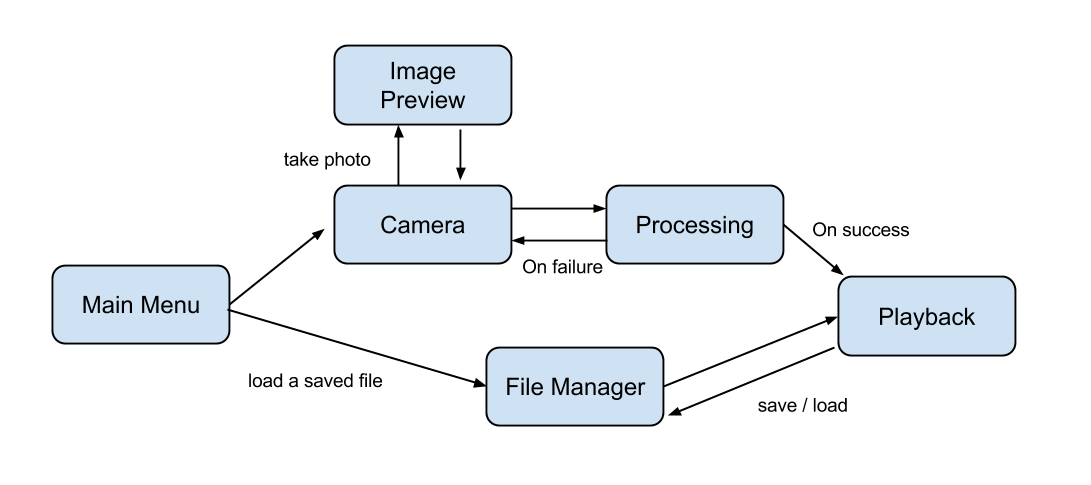
\includegraphics[width=150mm]{./assets/activitiesdiag.png}
                \caption{A flowchart of activities in the application}
                \label{image:activitydiag}
            \end{figure}

\subsubsection{Activity Layout}

The main activity for the app is SightReaderActivity. The app home screen has two options, Scan and Play.

[home screen capture] [Scan screen capture]

The Scan option launches the CameraActivity which takes you to the capture part of the app where you can take a picture of some sheet music. Tap the camera preview to take a picture, this launches the DisplayPhotoActivity which allows you to decide if you want to keep the picture or try again. You are then returned to the Camera preview screen. Once you have captured as many pictures as you want you tap done and the ProcessingActivity is called and the processing begin. Here we have a
processing screen as this can take some time to let the user know the app is still running.

[displayphotoactivity capture][progress screen capture]

The reason for using a new activity for each new action is that this allows each activity to handle normal function such as when the back button is pressed in the intuitive way. This is the recommended method of organising android apps as discussed in the background section.

The other option is to press ‘Play’ which takes you to the file management dialog. Here, you can view all of your previously processed pieces. Selecting a saved piece will then take you to the playback activity where you can hear it. This dialog is pre-configured to open in the default save file directory and has a filter to only show the relevant files.

We have used the FileDialog library, detailed in the background section, to implement this functionality.

\subsubsection{Camera Considerations}
We originally used the default android camera activity for taking the photographs, but later realised that we required additional features that this activity could not handle. Therefore, we implemented a new camera activity called SightReaderCameraView so that we could keep the theme of our app consistent and also have finer grained control on the camera options to maximise our detection accuracy.

\subsubsection{Saving Files}
\[Diagram here\] 
We need to save various files, both so the user can reaccess past music and also in order to deal with the limitations of device RAM.

\subsection{Music Detection - Overview}

Understanding sheet music is quite a complicated problem. The semantic meaning of the music is highly dependant on the relative locations of various features on the sheet. Understanding an English sentence is very simple, by contrast. Each letter is read sequentially from left to right, lines from top to bottom, and the spaces between letters denote words. When it comes to musical notation, however, even very small variations in the location of elements can entirely change the sound it
transcribes. This provides us with a significant challenge: we need precise and accurate detection methods if we want reliable results.

\subsubsection{Our Solution}

Broadly speaking the algorithm we created works as follows: 

\begin{enumerate}
\item{The photograph is taken and the images are rescaled and prepared for detection.}
\item{We pull out the staves from the image. They tell us where to look for the other features.}
\item{We sequentially extract each musical feature from the image, such as notes, clefs etc. Each pass can build on previous knowledge, eg. the beams between notes can take advantage of knowing the note locations.}
\item{We then use the relative locations of these features to determine the semantics of the musical piece.}
\end{enumerate}

Since there is no general way to detect an arbitrary feature using OpenCV, we had to try a wide variety of different methods based on our - admittedly small - prior knowledge of computer vision, what we learnt during first term, what we could find in different papers related to this question and what we could find in OpenCV tutorials. A detailed summary of the implementation of each step is explained below.

\subsection{Music Detection - Implementation details}

\subsubsection{Pre-processing}

As sheet music does not assign semantic meaning to colors, we decided to first remove all color from the image using a grayscale conversion. We then thresholded the image to increase image consistency in different lighting conditions. These processes are detailed in the background section.

Secondly, the convention in computer vision is to use white-on-black images. However, sheet music is the opposite, black markings on a white page. This means that before we do anything, we need to invert the image. This can be done very quickly by bitwise operations, ie. applying bitwise NOT to each pixel.

When we later transitioned from scanned pdf images onto real photographs we discovered a significant flaw with our preprocessing algorithm. On a photograph you are very likely to have shadows (including the shadow of the device taking the picture) and this means that some areas of the image are darker than others and therefore require a different threshold. We even found that on many images there did not even exist a single threshold value that could describe the entire
image. Therefore, we needed a method of finding the correct threshold dynamically.

(IMAGE) 

We solved this by first dividing the image into small, equal sized sections and found the average color of each section. As the image is going to be mostly black (a music sheet is mostly white space, and we have inverted the image) this means that features will be significantly lighter than this average. We therefore increase the average by a fixed percentage and use that as our threshold for that given section. Then, the sections are recombined back into a final binary image. We are now
ready to begin detecting features.

\subsubsection{Staves}

The staves are perhaps the single most important feature when it comes to detection.  All of the other elements on the page gain semantic meaning based on how they are placed relative to a stave. For example, notes determine their pitch based on their Y location on the stave lines. Therefore, we needed an accurate and robust detection method. We broke the problem into 2 halves, detecting all of the lines and then building the staves out of that pool of lines.

\paragraph{Detecting the lines}

Our first attempt to recognise the lines was to use the standard ‘Hough Lines’ algorithm. However, this approach had very serious problems with detecting the thin stave lines accurately, as explained in the background section.

After this obvious approach had failed, we decided to look into the literature and found that most previous work used a horizontal image projection to solve this particular problem (CIT). By horizontally projecting the image onto a single column of pixels, we could detect large horizontal lines on the page and from there extract the stave information. (IMAGE)

This proved simple to implement using OpenCV and served us very well for some time. We did not realise the fatal drawback to this approach until we moved from pdf images to images taken with a smartphone camera. 

\paragraph{Correcting Line Distortion}

On computer generated pdf images, the stave lines are always exactly horizontal and evenly spaced. This is how the horizontal projection can reliably extract the lines from all the surrounding noise. However, on a photograph this is an entirely unrealistic assumption. We identified 4 separate types of image distortion that undermine this algorithm’s effectiveness.

\begin{enumerate}
\item{Angular distortion when the camera is not perfectly aligned with the axes of the image.}
\item{Lens distortion from the camera causes slight bulging as you move towards the edge.}
\item{The paper may be slightly crumpled leading to sudden changes in line direction.}
\item{Perspective may lead to different lines having different degrees of distortion.}
\end{enumerate}

As all of the previous research has focused on scanned or generated images, we could not find a solution for distorted stave lines in the literature. We ultimately arrived at a novel solution (to our knowledge) for solving the issue, outlined as follows.

We first break the image down into several equal-sized vertical strips, similar to how a paper shredder works. The thinner a strip is, the lower the distortion is relative to the length of the line, and so below a certain width even moderately large distortion becomes negligible. We found that 30 strips offered a good compromise between accuracy and speed. Then, each of these thin strips have a horizontal projection performed on them. The line segments are
then extracted from these projections and are ‘threaded’ back together, by connecting lines on adjacent strips that are within a certain Y distance. Once the lines have been reconstructed, all viable lines (which are long enough to qualify) are saved. (IMAGE)

\paragraph{Building Staves from Lines}

The second half of the problem turned out to be much simpler. We had to take this pool of lines and extract staves, ie. groups of 5 lines with even spacing and width. This was done by sorting the lines vertically and then selecting each and every pair of lines. The pair was assumed to be the first 2 lines of the stave, and then the algorithm would check for 3 more lines with the same spacing below that pair. If all 5 lines are detected, the lines
are removed from the pool and saved as a stave.

An additional problem we found was that on pages with 5 or more staves, the algorithm could incorrectly detect a set of 5 equally spaced lines from different staves. For example, the first line of each of the 5 staves might be recognised as a stave itself. We solved this trivially by specifying a maximum spacing between stave lines. (IMAGE)


A final issue we ran into much later was that in cases where the image was at least moderately distorted, a single straight line could not accurately describe the location of a stave line on the paper, and so we had to keep the reconstructed lines from the detection algorithm rather than simply using their best-fit approximation. (IMAGE)

Now that we have a reliable method for detecting the staves, we can use this information greatly speed up the detection of other elements, by only looking in specific locations for them.  For example we know that a clef will only occur at the far left of a stave and so we only need to search a very small area of the page. It also allows us to give semantic meaning to many other musical features, such as determining the pitch of notes.

\subsubsection{Clef and time signature detection}

Despite their unique shape, clefs and time signatures do not have any particular characteristics that are easily exploitable to differentiate them, regardless of any eroding/dilating we may run first. This forced us to use a template matching algorithm to detect them. The way this is done is that we store an image for each feature that we want to detect - treble clef, bass clef, 4/4, 3/4, 2/4, 3/8, 6/8 time signatures, and run a separate
template match on each of these.

\paragraph{Extracting the results}

Although there is a clef at the beginning of each stave, and a time signature at the start of each music piece, there is a need to run the detection on the whole piece because additional clefs and signatures can be found at an arbitrary point in the staves.

The matrix ‘returned’ by \verb!matchTemplate! is of size:

\verb!(imageHeight - templateHeight + 1, imageWidth - templateWidth + 1)! .

Each cell of the matrix is an area of size one storing a double corresponding to the value computed in regards of the comparison method used at the given pixel location in the image. Since they are stored in arrays, results are difficult to extract directly using an intuitive algorithm. Fortunately,there exists a built-in method of OpenCV, \verb!minMaxLoc!, which returns an object storing the maximum and minimum value in the matrix of this type, as well as their respective locations - both are stored because depending on the comparison method used, the best results will be stored either at the maximum value location, or the minimum one.

With this method, we can extract a value that is then compared to a threshold, either calculated at the start of the method, or being set in terms of percentage of the first (therefore best) match, or a constant one if the comparison method is used in its normed way. If this value passes the threshold test, the associated location is a good match. The location is then added to the corresponding list (e.g. treble clefs list if we’re running the treble clef detection).

/* Proofreading needed for the next paragraph, not sure it actually means anything in English */

So far we have found the best match in the image. Unfortunately, the \verb!minMaxLoc! method does not remove the values from the matrix. We then have to set the values in the matrix to zero, at the just-found location but also around it to prevent another match just next to the previously found location, that would correspond to the same feature: we set all values in the areas around the point, in all directions and for the
size of the template image to zero, and iteratively run the extraction algorithm again until the threshold test fails. We have then found all features for the given method.



            \begin{figure}[ht!]
                \centering
                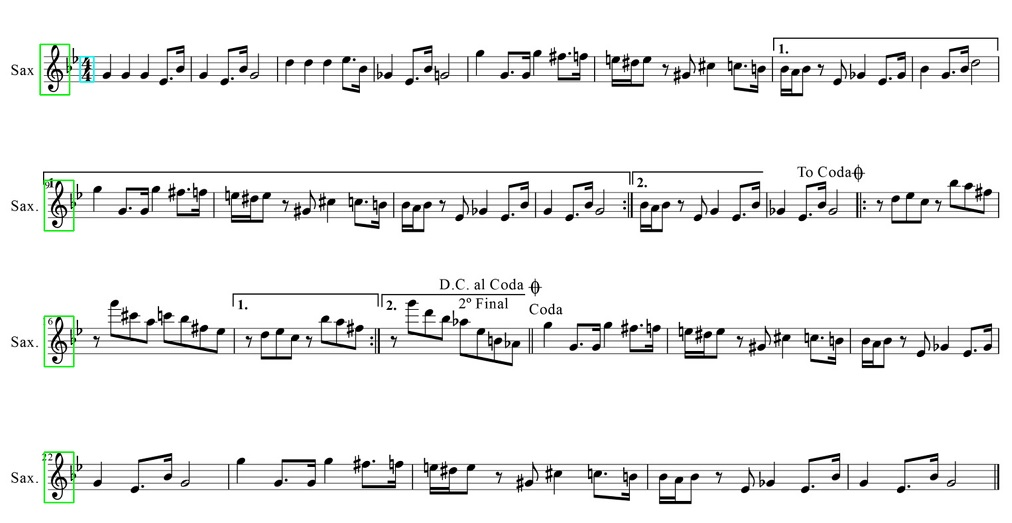
\includegraphics[width=1\textwidth]{./assets/detectedfeatures.jpg}
                \caption{All detected features through clefs and time signatures detection}
                \label{image:detectedfeatures}
            \end{figure}


Due to the uniqueness of their shapes, this gives excellent results in accuracy, with only 10\% of difference in the values between the best positive match and the worst positive match, and 45\% between the best positive match the best negative match. Unfortunately, it is also very time consuming with images this large, which is the reason we try to avoid using template matching as much as possible in the different
methods of detection.

\subsubsection{Crotchets}

There are many ways to detect crotchets. Unfortunately, most of them do not only recognise crotchets but also accidentals, beams, lyrics or sometimes just noise. We had to try many methods before finding a reliable one.

\paragraph{Hough Circles}

We originally tried to make use of the ‘Hough Circle’ algorithm. The method ‘HoughCircles’ is provided with OpenCV is very easy to use and merely depends on any variable: only the minimum distance between two detected circle centers is to be changed, as well as the minimum/maximum radius of the circles to detect. It was therefore quite straightforward to test the method. However, even when combined
with highlighting techniques like eroding/dilating, this did not give any consistent results. There was a high rate of both false positives and false negatives. Considering the processing time that it took to run HoughCircles, we decided not to go further in this direction and changed the algorithm.

\paragraph{Template matching}

Our first attempt was to use template matching. However, we quickly ran into a variety of non-trivial problems. Firstly, notes can have a tail either above or below its head, which would require us to use multiple templates. Additionally, the tails may not always be exactly vertical due to image distortion, which means we would either have to include even more templates, or risk sacrificing
detection quality by only matching against heads. Also, many features of sheet music look similar to note heads, as they are just a circular blob. This gave us a large nmber of false positives. Finally, different music notation programs use slightly different images for note heads, which would mean we need more templates still. Clearly, we needed a different approach.

\paragraph{FindContours}

We settled on the following algorithm: after a very careful and measured eroding, we used the built-in 'findContours' method to detect all contours. Because the 'findContours' method is very accurate, we need to have a measured eroding that would get rid of all the noise without erasing any of the notes. Fortunately, since notes are almost round and compact, we can afford a very large
eroding kernel, resulting in loads of features being simply erased, as well as all noise.
Once a contour has been found, we used moments to recover the center out of them, as explained in the background. This approach can very quickly and accurately detect every single note on the page, with almost no false positives. It is also highly insensitive to noise because of the large erosion kernel.
\begin{figure}[ht!]
    \centering
    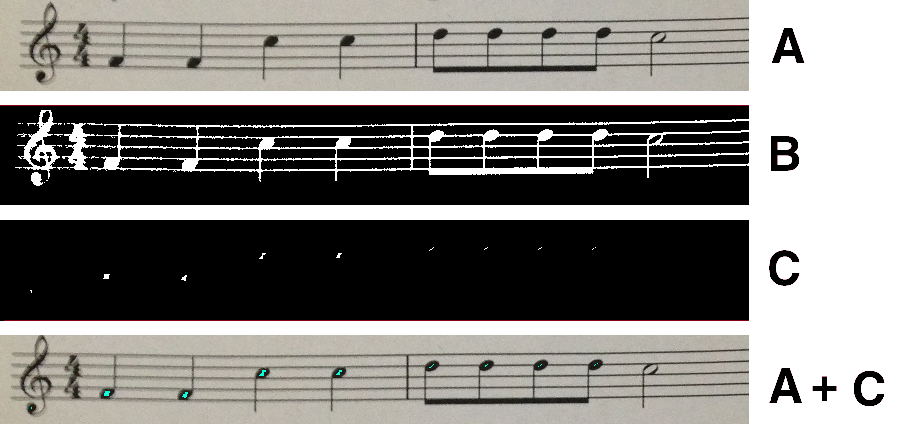
\includegraphics[width=1\textwidth]{./assets/highlight.png}
    \caption{Highlight of the computation of erosion for the purpose of crotchets detection}
    \label{image:highlight}
\end{figure}

We encountered some issues where beams would be mistaken for notes after the eroding, depending on the beam’s direction, slope, location and thickness.. Since it was sometimes very easy to mistake an eroded beam for a note, we also ran the same algorithm with a much lower erosion, leaving most of the beams intact. This allowed us to differentiate them from real notes,
catching the false positives. Notes are only recorded if they register as a note on both levels of erosion.

\begin{figure}[ht!]
    \centering
    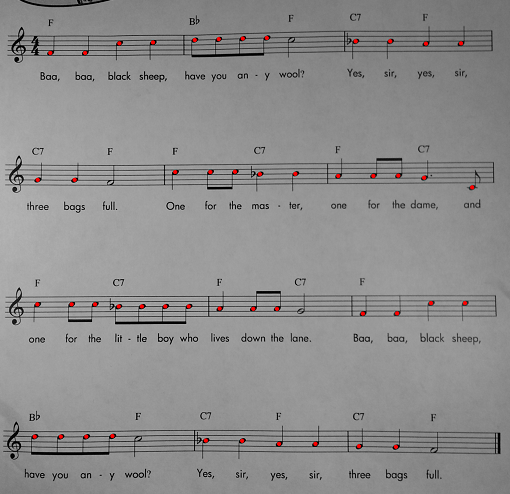
\includegraphics[width=1\textwidth]{./assets/crotchetsdetected.png}
    \caption{All detected crotchets are accurately detected through this algorithm}
    \label{image:crotchetsdetected}
\end{figure}

The notes are then ordered by x coordinate, which aids the detection of some of the following features.

\subsubsection{Accidentals}

Similarly to clefs, the uncharacterised shapes of accidentals forces the use of template matching. But as opposed to clefs, we need not run the detection on the whole stave: we just run it on areas around the note, not too specific because of noise, small location errors and the actual position before the note which is not fixed, depending on the actual
position of the note and that of the neighbouring notes. Therefore, we run the template matching method on a fixed small area in front of each note.

\subsubsection{Beams}

At first glance, beam detection may appear similar to stave detection. However, they are not necessarily horizontal which makes a horizontal projection impractical. Fortunately we can exploit the fact that they are very thick instead (compared to all other lines in sheet music).

First, we eroded the image to get rid of the small noise and stave lines which may interfere with detecting beams. We then used Hough lines to try and detect the remaining lines, naming only the beam lines. Unfortunately, we ran into the problem where Hough lines cannot detect lines of significantly differing sizes, as explained in the background. Due to the
significant processing overhead it introduced, we decided to find another approach.

First, we applied a strong erosion to the image. This left us with only the most prominent features, namely the notes and beams. Then, using our prior knowledge of the location of notes, we black out all notes on the eroded image, leaving us with just beams.

From here, we apply a vertical projection to the image, which picks out the x-dimension ranges of beams. Now that we know the x locations, for each x range we extract its vertical strip from the eroded image and we then perform a horizontal projection to also find their y locations.

There is an additional problem to consider, double beams are a common feature in sheet music and we wanted to support their detection. However, some of these double beams may be quite small as shown in \ref{image:beamsdetected} 


We solved this by taking the eroded image, after the first pass of the algorithm, and blacking out all the beams we detected in that pass. Then the detection can be run again to find the second beam in a double beam. This can be repeated again for triple beams and so on.


\begin{figure}[h!]
    \centering
    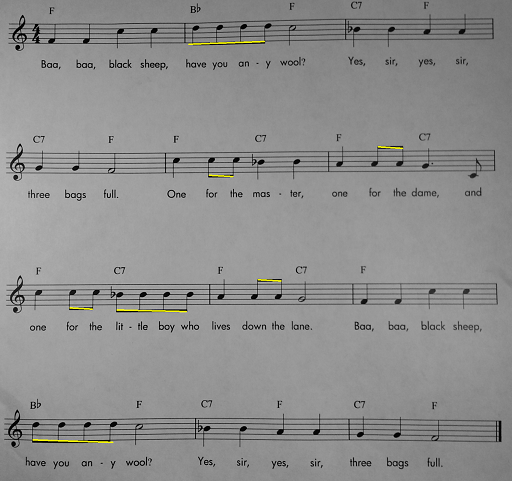
\includegraphics[width=1\textwidth]{./assets/beamsdetected.png}
    \caption{All detected beams after running the method}
    \label{image:beamsdetected}
\end{figure}

\subsubsection{Quavers}

We do not check for quavers directly, rather we perform an extra check on each crochet to determine if it is next to a quaver tail. This is a 2-part process: first, we erode the image with a non-square kernel of width 2. This will erase the stave lines but keep the details of every feature with width greater than 2 pixels; which includes
quavers. We then isolate a small area to the right of the note and use the ‘findContours’ algorithm on this area. If a contour is detected that is tall enough to be considered a quaver tail rather than noise, we record that the note is a quaver.

\subsubsection{Dots}

The only robust way to accurately detect dots is to use the findContours on some area after note, after some eroding, and check for the location of the center of gravity of the contours if it isn’t too wide or high, the same way we did for crotchets. This value is then compared to the expected location: the exact middle of
the stavelines. The difference in height is computed, using the accurate exact value of the stave positions at the given location. If it is small enough, the contour is validated as a dot, and the duration of the note is updated.

Contours are well suited to this problem as dots necessarily have a border of white space around them - otherwise they would not be a dot.

\begin{figure}[ht!]
    \centering
    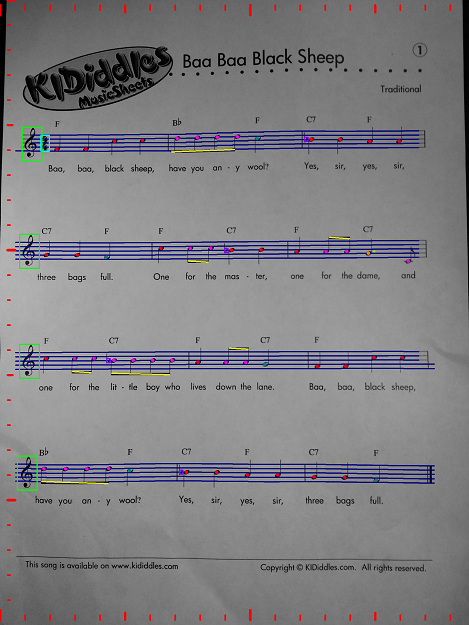
\includegraphics[width=1\textwidth]{./assets/detected.png}
    \caption{All detected features after running the whole application. For debugging purposes, a scale is printed as well. Each note color corresponds to a different duration of the note.}
    \label{image:detected}
\end{figure}

\subsection{Interpretation and Playback}
\subsubsection{Intermediary representation}
Once the music has been detected, we build up an intermediary representation of the piece. The structure of this representation is as follows:
The \verb!Piece! class holds information such as the clef, tempo and time signature of the piece. \verb!Piece!s contain a list of \verb!Bar!s, which themselves are lists of \verb!Chord!s, and a \verb!Chord! is a list of \verb!AbstractNote!s. There are then two subclasses of \verb!AbstractNote! - \verb!PlayedNote! and \verb!RestNote!. Notes contained information about their pitch, duration and velocity. We felt this intermediary representation was adequate for our immediate needs, but it was also open to any potential extensions we may desire later on.

\subsubsection{Playback}
Playback was achieved in two steps. First we generated a MIDI file from our intermediary representation. This was a case of iterating through the nested lists using the helper functions provided by the Android MIDI Library. This library provided an interface to the MIDI format through the class \verb!MidiFile!, which represented a series of \verb!MidiTrack!s. Tracks were manipulated by inserting events, and
a function \verb!MidiTrack.insertNote()! meant inserting either a rest or played note was straightforward. Once generated it was saved to the device.  [] once retrieved from the file system, it was played back using the Android JetPlayer Class.

